\documentclass[final,3p]{elsarticle}

% \documentclass[preprint,12pt]{elsarticle}

%% Use the option review to obtain double line spacing
%% \documentclass[authoryear,preprint,review,12pt]{elsarticle}

%% Use the options 1p,twocolumn; 3p; 3p,twocolumn; 5p; or 5p,twocolumn
%% for a journal layout:
% \documentclass[final,1p,times]{elsarticle}
%% \documentclass[final,1p,times,twocolumn]{elsarticle}
% \documentclass[final,3p,times]{elsarticle}
%% \documentclass[final,3p,times,twocolumn]{elsarticle}
% \documentclass[final,5p,times]{elsarticle}
%% \documentclass[final,5p,times,twocolumn]{elsarticle}
\usepackage[portuguese]{babel}

%% For including figures, graphicx.sty has been loaded in
%% elsarticle.cls. If you prefer to use the old commands
%% please give \usepackage{epsfig}

%% The amssymb package provides various useful mathematical symbols
\usepackage{amssymb}
\usepackage{amsmath}
\usepackage{multirow}

\usepackage{subfigure}

\usepackage{pgfplots}
\pgfplotsset{compat=1.18}
\usepgfplotslibrary{statistics}
\usepackage{pgfplotstable}

\usepackage{placeins}
\usepackage{hyperref}
\numberwithin{equation}{section}

\usepackage{algorithm}
\usepackage[noEnd=true, indLines=true]{algpseudocodex}
\algrenewcommand\algorithmicrequire{\textbf{Entrada:}}
\algrenewcommand\algorithmicwhile{\textbf{Enquanto}}
\algrenewcommand\algorithmicrepeat{\textbf{Repete}}
\algrenewcommand\algorithmicuntil{\textbf{Até}}
\algrenewcommand\algorithmicif{\textbf{Se}}
\algrenewcommand\algorithmicthen{\textbf{então}}
\algrenewcommand\algorithmicelse{\textbf{Caso contrário}}
\algrenewcommand\algorithmicensure{\textbf{Objetivo:}}
\algrenewcommand\algorithmicreturn{\textbf{Retorna:}}
\algrenewcommand\algorithmicdo{\textbf{faça}}
\algrenewcommand\algorithmicforall{\textbf{Para todos}}
\algnewcommand{\LineComment}[1]{\State \(\triangleright\) \textcolor{black!50}{\emph{#1}}}

% \usepackage[fleqn]{nccmath}
% \usepackage{multicol}


%=========== Gloabal Tikz settings
% \pgfplotsset{compat=newest}
% \usetikzlibrary{math}
% \pgfplotsset{
%     height = 10cm,
%     width = 10cm,
%     tick pos = left,
%     legend style={at={(0.98,0.30)}, anchor=east},
%     legend cell align=left,
%     }
%  \pgfkeys{
%     /pgf/number format/.cd,
%     fixed,
%     precision = 1,
%     set thousands separator = {}
% }

%% The amsthm package provides extended theorem environments
%% \usepackage{amsthm}

%% The lineno packages adds line numbers. Start line numbering with
%% \begin{linenumbers}, end it with \end{linenumbers}. Or switch it on
%% for the whole article with \linenumbers.
%% \usepackage{lineno}

\usepackage{listings}
\usepackage{xcolor}

\definecolor{codegreen}{rgb}{0,0.6,0}
\definecolor{codegray}{rgb}{0.5,0.5,0.5}
\definecolor{codepurple}{rgb}{0.58,0,0.82}
\definecolor{backcolour}{rgb}{0.98,0.98,0.98}

\lstdefinestyle{mystyle}{
    backgroundcolor=\color{backcolour},
    commentstyle=\color{codegreen},
    keywordstyle=\color{magenta},
    numberstyle=\tiny\color{codegray},
    stringstyle=\color{codepurple},
    basicstyle=\ttfamily\footnotesize,
    breakatwhitespace=false,
    breaklines=true,
    captionpos=b,
    keepspaces=true,
    numbers=left,
    numbersep=5pt,
    showspaces=false,
    showstringspaces=false,
    showtabs=false,
    tabsize=2
}

\lstset{style=mystyle}

% \journal{Nuclear Physics B}

\begin{document}

\begin{frontmatter}

%% Title, authors and addresses

%% use the tnoteref command within \title for footnotes;
%% use the tnotetext command for theassociated footnote;
%% use the fnref command within \author or \address for footnotes;
%% use the fntext command for theassociated footnote;
%% use the corref command within \author for corresponding author footnotes;
%% use the cortext command for theassociated footnote;
%% use the ead command for the email address,
%% and the form \ead[url] for the home page:
%% \title{Title\tnoteref{label1}}
%% \tnotetext[label1]{}
%% \author{Name\corref{cor1}\fnref{label2}}
%% \ead{email address}
%% \ead[url]{home page}
%% \fntext[label2]{}
%% \cortext[cor1]{}
%% \affiliation{organization={},
%%             addressline={},
%%             city={},
%%             postcode={},
%%             state={},
%%             country={}}
%% \fntext[label3]{}

\title{Estimativa do Ponto de Operação de um Sistema de Produção Simples\tnoteref{label_title}}
\tnotetext[label_title]{Relatório número 1 como parte dos requisitos da disciplina PP590: Tópicos em Geoengenharia de Reservatórios.}

%% use optional labels to link authors explicitly to addresses:
%% \author[label1,label2]{}
%% \affiliation[label1]{organization={},
%%             addressline={},
%%             city={},
%%             postcode={},
%%             state={},
%%             country={}}
%%
%% \affiliation[label2]{organization={},
%%             addressline={},
%%             city={},
%%             postcode={},
%%             state={},
%%             country={}}

\author{Tiago C. A. Amorim\fnref{label_author}}
\tnotetext[label_author]{Atualmente cursando doutorado no Departamento de Engenharia de Petróleo da Faculdade de Engenharia Mecânica da UNICAMP (Campinas/SP, Brasil).}
\ead{t100675@dac.unicamp.br}
\affiliation[Tiago C. A. Amorim]{organization={Petrobras},%Department and Organization
addressline={Av. Henrique Valadares, 28},
city={Rio de Janeiro},
postcode={20231-030},
state={RJ},
country={Brasil}}

\begin{abstract}
    Foi desenvolvido em Python um sistema para realizar a estimativa da perda de carga ao longo de um poço produtor satélite. Os testes realizados mostraram que, para as condições avaliadas, é possível conseguir bons resultados com poucas subdivisões dos elementos descritos.
\end{abstract}


%%Graphical abstract
% \begin{graphicalabstract}
%\includegraphics{grabs}
% \end{graphicalabstract}

%%Research highlights
% \begin{highlights}
% \item Research highlight 1
% \item Research highlight 2
% \end{highlights}

\begin{keyword}
    Modelo integrado \sep Correlações Black-Oil
%% keywords here, in the form: keyword \sep keyword

%% PACS codes here, in the form: \PACS code \sep code

%% MSC codes here, in the form: \MSC code \sep code
%% or \MSC[2008] code \sep code (2000 is the default)

\end{keyword}

\end{frontmatter}

%% \linenumbers

%% main text
\section{Introdução}

    Este relatório descreve os principais elementos desenvolvidos para resolver o exercício número 1 proposto na 1$^a$ aula de Tópicos em Geoengenharia de Reservatórios.

\section{Metodologia}

    \subsection{Problema Proposto}

        Foi proposto encontrar o ponto de operação de um poço produtor de óleo conectado diretamente a uma unidade de produção (configuração \emph{satélite}). Pela descrição na figura \ref{fig:problema_proposto} observa-se que:

        \begin{itemize}
            \item O problema é isotérmico: serão ignoradas as trocas térmicas na formulação.
            \item O óleo é muito subsaturado: todas as equações desenvolvidas irão considerar que não existe gás livre ao longo da tubulação.
        \end{itemize}

        \begin{figure}
            \centering
            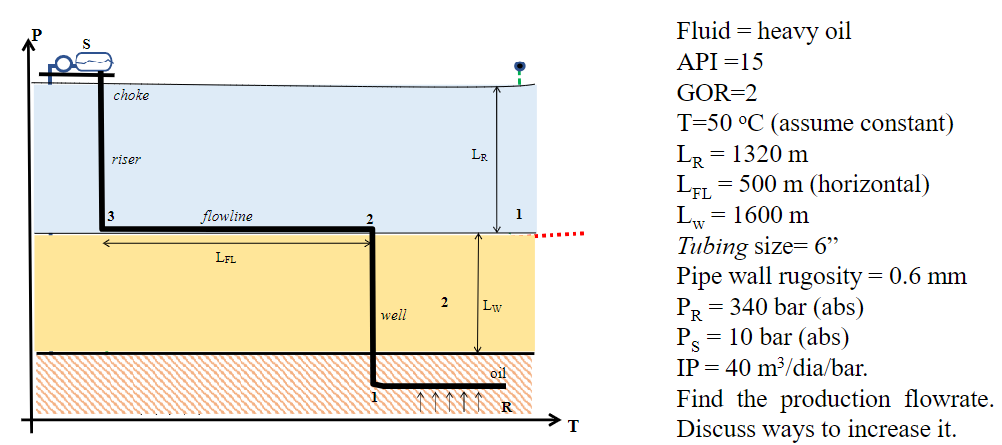
\includegraphics[width=0.8\textwidth]{Problem_01.png}
            \caption{Problema proposto número 1.}
            \label{fig:problema_proposto}
        \end{figure}

        Toda a resolução do problema foi feita em \texttt{Python}. Foram criados módulos específicos para cada elemento integrante do problema proposto. Dentro de cada módulo um ou mais objetos foram construídos. O código mais atual pode ser encontrado em \href{https://github.com/TiagoCAAmorim/IntegratedModel/tree/main/sample}{https://github.com/TiagoCAAmorim/IntegratedModel}.

    \subsection{Correlações Black-Oil \emph{(Módulo \texttt{pvt.py})}}

        Para este problema todas a propriedades de óleo foram estimadas a partir de correlações \emph{clássicas}:

        \begin{itemize}
            \item Pressão de bolha, fator volume de formação do óleo na pressão de bolha e viscosidade por Standing \cite{standing1952volumetric}.
            \item Compressibilidade do óleo na pressão de bolha por Vasquez e Beggs \cite{VasquezBeggs}.
        \end{itemize}

        Não foram necessárias para resolver o problema proposto, mas também foram implementadas correlações para cálculo de propriedades de gás (z, Bg) com correlações de Standing.

        Dentro do módulo \texttt{pvt.py} existe a descrição de um objeto: \textbf{PVT}. O usuário precisa informar algumas informações básicas (api, pressão, temperatura, dg etc.) e pode usar as rotinas desenvolvidas para calcular outras propriedades com as correlações. Uma forma de avaliar a implementação foi refazer os mesmos gráficos que foram apresentados em aula \cite{aula01} (Figuras \ref{fig:grid_pvt} e \ref{fig:grid_pvt_gas}).

        \begin{figure}
            \centering
            \subfigure[Razão de solubilidade para diferentes parâmetros.]{
              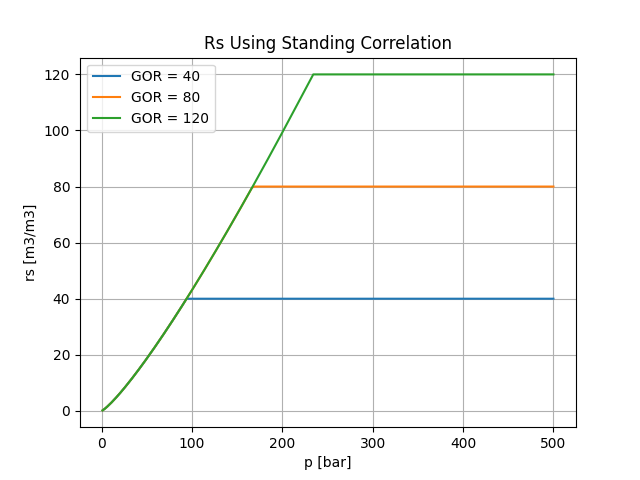
\includegraphics[width=0.45\textwidth]{pvt/rs.png}
            }
            \subfigure[Pressão de bolha pela correlação de Standing e invertendo a correlação de razão de solubilidade.]{
              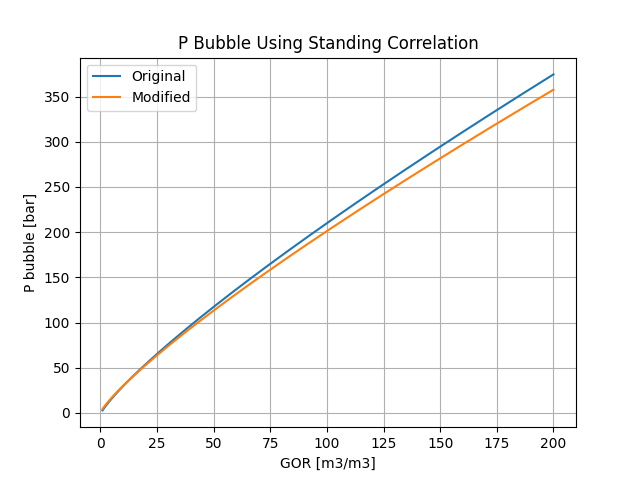
\includegraphics[width=0.45\textwidth]{pvt/p_bubble.png}
            } \label{subfig:imagea}

            \subfigure[Pressão de bolha para diferentes parâmetros.]{
              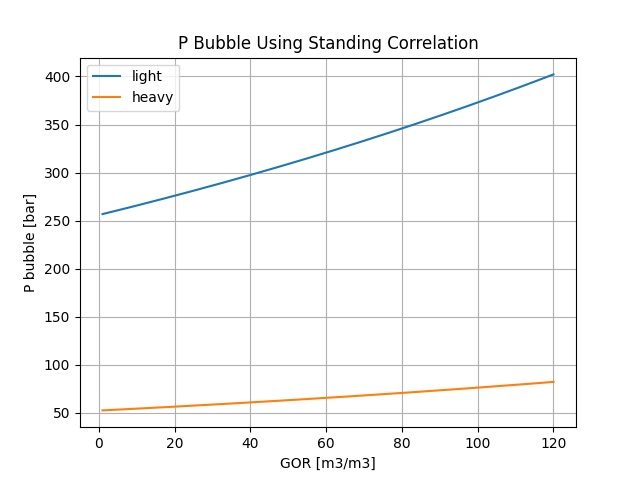
\includegraphics[width=0.45\textwidth]{pvt/p_bubble2.png}
            }
            \subfigure[Fator volume de formação do óleo para diferentes parâmetros.]{
              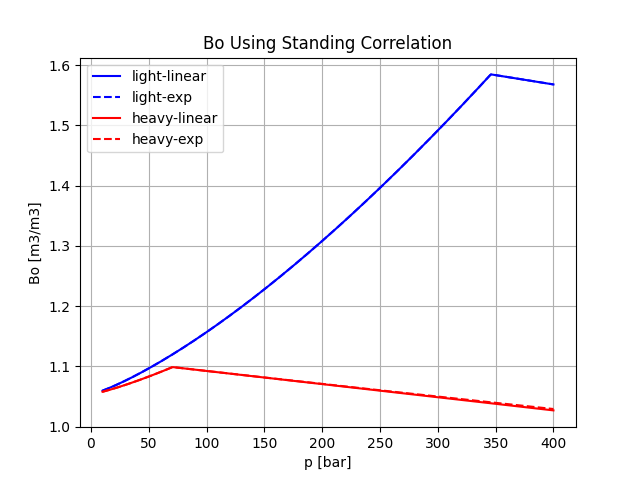
\includegraphics[width=0.45\textwidth]{pvt/bo.png}
            }

            \subfigure[Densidade do óleo para diferentes parâmetros.]{
              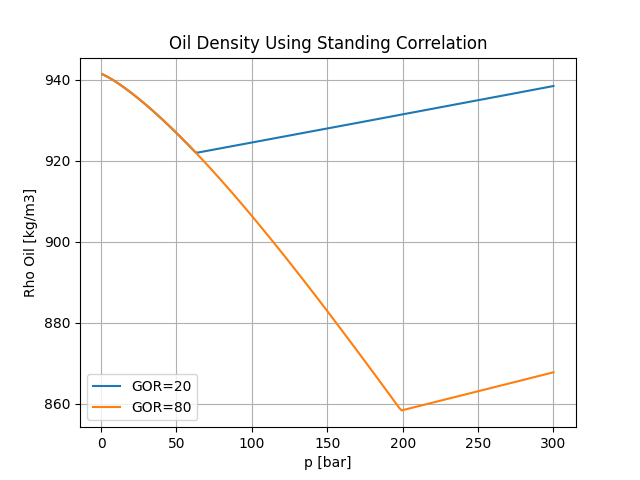
\includegraphics[width=0.45\textwidth]{pvt/rhoo.png}
            }
            \subfigure[Viscosidade do óleo para diferentes parâmetros.]{
              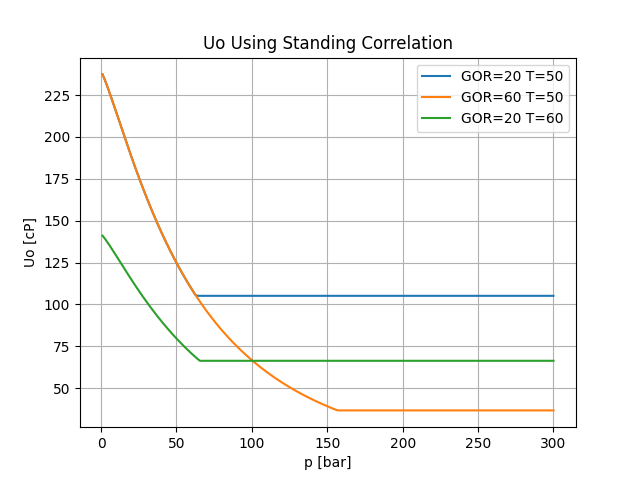
\includegraphics[width=0.45\textwidth]{pvt/uo.png}
            }

            \caption{Variação de propriedades de óleo com as correlações implementadas.}
            \label{fig:gridpvt}
          \end{figure}


        \begin{figure}
            \centering
            \subfigure[Densidade do gás para diferentes parâmetros.]{
              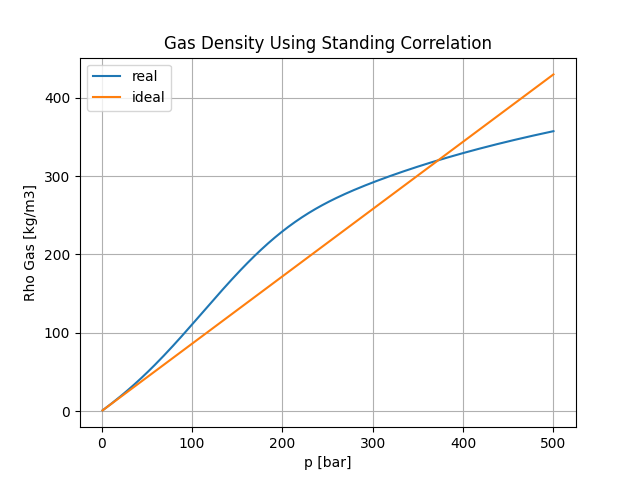
\includegraphics[width=0.45\textwidth]{pvt/rhog.png}
            }
            \subfigure[Fator volume de formação do gás para diferentes parâmetros.]{
              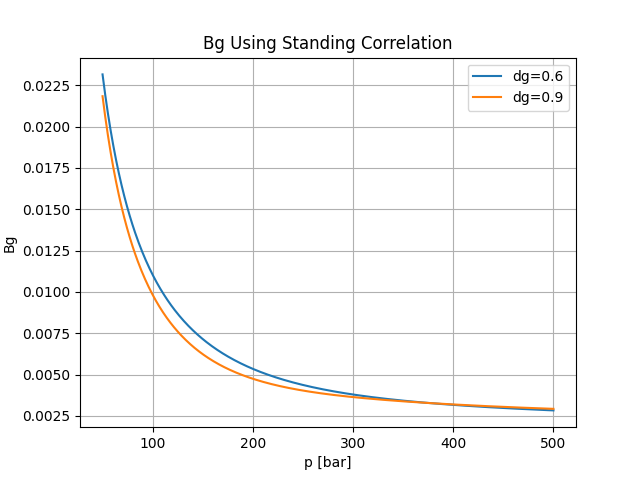
\includegraphics[width=0.45\textwidth]{pvt/bg.png}
            }
            \subfigure[Parâmetros z do gás para diferentes parâmetros.]{
              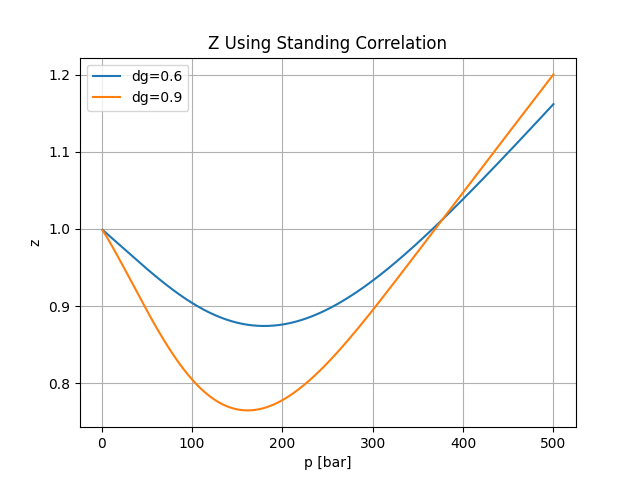
\includegraphics[width=0.45\textwidth]{pvt/z.png}
            }

            \caption{Variação de propriedades de gás com as correlações implementadas.}
            \label{fig:grid_pvt_gas}
          \end{figure}

          Observa-se que existe um desvio entre a correlação de Standing para pressão de bolha e a inversão da correlação de razão de solubilidade (figura \subref{subfig:imagea}). Para manter coerência entre as diferentes estimativas, optou-se por utilizar \emph{por padrão} no cálculo da pressão de boha a fórmula invertida a partir da correlação de razão de solubilidade. O usuário ainda tem acesso à correlação original de Standing.

          Para o problema proposto é informado um fluido de baixa razão gás-óleo. Como a pressão de bolha deste fluido (11.83 bar) é muito próxima da menor pressão do sistema a ser modelado (10 bar), será possível ter uma boa estimativa considerando apenas óleo no sistema. Um problema que aparece é o comportamento do fator volume de formação ($Bo$), pois o fluido estará submetido a uma pressão muito maior que a sua pressão de bolha. Foi avaliado o efeito de considerar a forma \emph{exponencial} de cálculo do $Bo$, ao invés de usar a forma \emph{linear}, que é uma aproximação da primeira (). Observa-se que para o fluido do problema proposto existe uma variação no $Bo$ em função da formulação utilizada (figura \ref{fig:bo_problema_proposto}), mas não é significativa. Para fluidos menos subsaturados a diferença é ainda menor (figura ).

          \begin{figure}
            \centering
            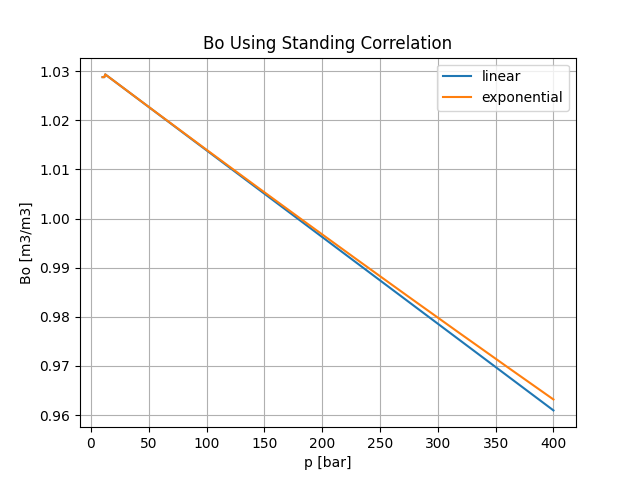
\includegraphics[width=0.45\textwidth]{pvt/bo2.png}
            \caption{Estimativa de fator voluma de formação para o fluido do problema proposto.}
            \label{fig:bo_problema_proposto}
        \end{figure}


    %     Um dos modelos de aquífero analítico mais difundidos é o de Fetkovich \cite{schlumberger2009technical} \cite{computer2022cmg} \cite{rosa2006engenharia}. O método de Fetkovich se baseia em um modelo transiente, e em muitos casos se aproxima das respostas do método de van Everdingen-Hurst \cite{VanEverdingen-Hurst}. A vantagem do método de Fetkovich é a simplicidade de sua aplicação, pois não depende de técnicas de superposição.

    %     O modelo de Fetkovich assume que a contribuição de um aquífero pode ser adequadamente modelada por um índice de produtividade, ou seja, que o influxo de água do aquífero para o reservatório é diretamente proporcional à diferença entre a pressão média do aquífero e a pressão na interface entre o reservatório e o aquífero \cite{fetkovich1971simplified}. O método negligencia quaisquer efeitos transientes no aquífero. O efeito desta premissa será maior em casos onde existe uma \emph{rápida} variação na pressão na interface entre o reservatório e o aquífero, fazendo com que os resultados do método de Fetkovich se desviem dos resultados mais rigorosos do método de van Everdingen-Hurst \cite{AHMED2019663}. Para problemas em que a variação desta pressão é mais gradual, o método de Fetkovich apresenta bons resultados.

    %     O método primeiramente assume um índice de produtividade constante para o aquífero:

    %     \begin{align}
    %         Q_w = \frac{dW_e}{dt} = J (p_{aq} - p_{res})& \label{eq:j}
    %     \end{align}

    %     A equação de balanço de massa assume que a compressibilidade do aquífero é constante, e que a depleção é proporcional à redução do volume de água:

    %     \begin{align}
    %         W_e = c_{aq} W_{i,aq} (p_{i,aq} - p_{aq})& \label{eq:compAquif}
    %     \end{align}

    %     A partir de \ref{eq:compAquif} é possível encontrar uma equação para a pressão média do aquífero:

    %     \begin{align}
    %         p_{aq} &= p_{i,aq} \left( 1 - \frac{W_e}{c_{aq} W_{i,aq} p_{i,aq}} \right) \nonumber \\
    %         &= p_{i,aq} \left( 1 - \frac{W_e}{W_{e,max}} \right) \label{eq:pAquif}
    %     \end{align}

    %     Diferenciando \ref{eq:pAquif} no tempo:

    %     \begin{align}
    %         \frac{dp_{aq}}{dt} &= - \frac{p_{i,aq}}{W_{e,max}} \frac{dW_e}{dt} \label{eq:dpaqdt}
    %     \end{align}

    %     Isolando $p_{aq}$ em \ref{eq:j} e diferenciando no tempo:

    %     \begin{align}
    %         \frac{dp_{aq}}{dt} &= \frac{1}{J} \frac{d^2W_e}{dt^2} + \frac{dp_{res}}{dt} \label{eq:dpaqdt2}
    %     \end{align}

    %     Igualando \ref{eq:dpaqdt} e \ref{eq:dpaqdt2}:

    %     \begin{align}
    %         \frac{d^2W_e}{dt^2} &= - \frac{J p_{i,aq}}{W_{e,max}} \frac{dW_e}{dt} - J \frac{dp_{res}}{dt} \label{eq:dwe2dt2}
    %     \end{align}

    %     Assumindo uma pressão constante na interface entre o aquífero e o reservatório ($\frac{dp_{res}}{dt} = 0$) e lembrando que $p_{aq}(t=0)=p_{i,aq}$, é possível resolver a EDO \ref{eq:dwe2dt2}:

    %     \begin{align}
    %         \frac{dW_e}{dt} &= J (p_{i,aq} - p_{res}) e^{\frac{J p_{i,aq}}{W_{e,max}} t} \label{eq:dwedt}
    %     \end{align}

    %     Integrando \ref{eq:dwedt} no tempo com $W_e(t=0)=0$:

    %     \begin{align}
    %         W_e &= \frac{W_{e,max}}{p_{i,aq}} (p_{i,aq} - p_{res}) \left( 1- e^{\frac{J p_{i,aq}}{W_{e,max}} t} \right) \label{eq:we}
    %     \end{align}

    %     Como a suposição de pressão constante na interface entre o aquífero e o reservatório é muito forte, Fetkovich propõe aplicar \ref{eq:we} de maneira incremental. Para um tempo $t_j$ com $j=1,2,\ldots,n$:

    %     \begin{align}
    %         (\Delta W_e)_j &= \frac{W_{e,max}}{p_{i,aq}} ((\overline{p}_{i,aq})_{j-1} - (\overline{p}_{res})_j) \left( 1- e^{\frac{J p_{i,aq}}{W_{e,max}} \Delta t_j} \right) \label{eq:deltawe}
    %     \end{align}

    %     \noindent
    %     onde

    %     \begin{align}
    %         (\overline{p}_{res})_j &= \frac{(p_{res})_j + (p_{res})_{j-1}}{2} \label{eq:presmedio}
    %     \end{align}

    %     \begin{align}
    %         (\overline{p}_{i,aq})_j &= p_{i,aq} \left( 1 - \frac{(\Delta W_e)_j}{W_{e,max}} \right) \label{eq:paqmedio}
    %     \end{align}

    %     Com $(p_{res})_0 = p_{i,res}$ e $(\overline{p}_{i,aq})_0 = p_{i,aq}$.

    %     Ao final do procedimento, o volume de água que passa do aquífero ao reservatório é a soma dos incrementos:

    %     \begin{align}
    %         W_e = \sum_{j = 1}^{n}  (\Delta W_e)_j \label{eq:wetotal}
    %     \end{align}

    %     O termo da pressão no aquífero é calculado no passo de tempo anterior. O único termo que não pode ser calculado diretamente é $(p_{res})_j$. Como este termo é normalmente função, entre outros, do influxo de água ($\sum_{j} (\Delta W_e)_j$), a cada passo de tempo é preciso resolver um problema do tipo $y = g(y)$.

    % \subsection{Método de Euler}

    %     O objetivo do método de Euler é encontrar uma aproximação da solução de um problema de valor inicial bem posto (PVI):

    %     \begin{align}
    %         \frac{dy}{dt} = f(t,y), \quad a \leq t \leq b, \quad y(a) = \alpha \label{eq:pvi}
    %     \end{align}

    %     É possível usar o Teorema de Taylor para estimar o valor de $y(t_{j+1})$ a partir do valor de $y(t_j)$. Assumindo $y(t_{j+1}) - y(t_j) = h$ e com $\xi_j \; \epsilon \; (t_j, t_{j+1})$:

    %     \begin{align}
    %         y(t_{j+1}) = y(t_j) + h \left. \frac{dy}{dt} \right|_{t_j} + \frac{h^2}{2} \left. \frac{d^2y}{dt^2} \right|_{\xi_j} \label{eq:taylor}
    %     \end{align}

    %     Substituindo \ref{eq:pvi} em \ref{eq:taylor} e ignorando o resto, chega-se ao método de Euler. Fazendo $w_j \approx y(t_j)$, aplicando a discretização em $t$ em $n$ passos e a condição inicial:

    %     \begin{align}
    %         h &= \frac{b-a}{n} \nonumber \\
    %         t_j &= a + h j \nonumber \\
    %         w_0 &= \alpha \nonumber \\
    %         w_j &= w_{j-1} + h f(t_{j-1}, w_{j-1}) \label{eq:euler}
    %     \end{align}

    %     É possível mostrar que o limitante do erro do método de Euler é dado por\footnote{Prova completa em \cite{burden2016analise}}:

    %     \begin{align}
    %         \left\lvert y(t_j) - w_j \right\rvert &\leq \frac{h M}{2 L} \left[ e^{L(t_j-t_0)} -1 \right]  \label{eq:limitante}
    %     \end{align}

    %     \noindent
    %     onde

    %     \begin{align}
    %         \left\lvert \frac{\partial f}{\partial y} (t,y(t)) \right\rvert &\leq L \label{eq:L} \\
    %         \left\lvert \frac{d^2y}{dt^2} (t) \right\rvert = \left\lvert \frac{df}{dt} (t,y(t)) \right\rvert =& \nonumber \\
    %         \left\lvert \frac{\partial f}{\partial t} (t,y(t)) + \frac{\partial f}{\partial y} (t,y(t)) f(t,y(t)) \right\rvert &\leq M \label{eq:M}
    %     \end{align}

    %     A estimativa do limitante do erro pode ser feita mesmo sem conhecer explicitamente a função $y(t)$. Neste caso os valores de $L$ e $M$ serão estimados com os valores aproximados $w_j$.

    %     \subsection{Modelo de Fetkovich como PVI}

    %     Uma forma de resolver o modelo proposto por Fetkovich sem ter que assumir uma pressão constante na interface entre o aquífero e o reservatório é transformá-lo em um problema de valor inicial.

    %     Vamos assumir um modelo simples de reservatório em que é alcançado equilíbrio hidrostático \emph{instantaneamente}\footnote{Em um instante qualquer todo o reservatório estará na mesma pressão $p_{res}$.}. Por simplicidade é assumido que $Bw=1$.

    %     \begin{align}
    %         N Bo + W_{res} = Pv  \label{eq:reservatorio}
    %     \end{align}

    %     Serão assumidas correlações lineares do fator volume de formação do óleo com a pressão, e do volume poroso com a pressão.

    %     \begin{align}
    %         N Bo_b [1+c_{o,b}(p_b-p_{res})] &+ W_{res} = \nonumber \\
    %         & Pv_i [1 - c_r (p_{i,res} - p_{res})]  \label{eq:reservatorio2}
    %     \end{align}

    %     Isolando $p_{res}$ em \ref{eq:reservatorio2}:

    %     \begin{align}
    %         p_{res} = \frac{N Bo_b (1+c_{o,b} p_b) + W_{res} - Pv_i (1 - c_r p_{i,res})}
    %         {N Bo_b c_{o,b} + Pv_i c_r }  \label{eq:pres}
    %     \end{align}

    %     Derivando \ref{eq:pres} no tempo:

    %     \begin{align}
    %         \frac{dp_{res}}{dt} =& \frac{\frac{dN}{dt} Bo_b (1+c_{o,b} p_b) + \frac{dW_{res}}{dt}}
    %         {N Bo_b c_{o,b} + Pv_i c_r} + \nonumber \\
    %         & -p_{res}\frac{\frac{dN}{dt} Bo_b c_{o,b}}{N Bo_b c_{o,b} + Pv_i c_r} \label{eq:dpresdt}
    %     \end{align}

    %     Substituindo \ref{eq:dpresdt} em \ref{eq:dwe2dt2}, e assumindo $\frac{dN}{dt} = f(t,p_{res})$, encontra-se um PVI da forma:

    %     \begin{align}
    %         \frac{d^2y}{dt^2} = -\alpha \frac{dy}{dt} - f(t,y), \quad a \leq t \leq b, \quad y(a) = \alpha \label{eq:pvi2}
    %     \end{align}


    %     Para aplicar o método de Euler será preciso focar no caso específico em que não há produção de óleo ($\frac{dN}{dt} = 0$):

    %     \begin{align}
    %         \frac{d^2W_e}{dt^2} &= - J \left(\frac{p_{i,aq}}{W_{e,max}} + \frac{1}{N Bo_b c_{o,b} + Pv_i c_r} \right)  \frac{dW_e}{dt} \label{eq:dwe2dt2res}
    %     \end{align}

    %     Como a condição inicial de $p_{aq}(t=0)=p_{i,aq}$ se mantém, a EDO \ref{eq:dwe2dt2res} tem solução analítica análoga a \ref{eq:dwedt}:

    %     \begin{align}
    %         \frac{dW_e}{dt} &= J (p_{i,aq} - p_{res}) e^{J \left( \frac{p_{i,aq}}{W_{e,max}} + \frac{1}{N Bo_b c_{o,b} + Pv_i c_r} \right)  t} \label{eq:dwedtres}
    %     \end{align}

    %     Desta forma será possível comparar a resposta exata (\ref{eq:dwedtres}) com as aproximações do método de Fetkovich (\ref{eq:deltawe}) e do método de Euler (\ref{eq:dwe2dt2res}).


\section{Implementação} \label{sec:implementacao}

        Todo o código utilizado nesta análise foi desenvolvido em C++. Foram criados objetos próprios para cada elemento integrante do problema proposto:

        % \begin{description}
        %     \item[IVP] Classe que define um problema de valor inicial na forma \ref{eq:pvi}.
        %     \begin{itemize}
        %         \item O usuário precisa especificar $f(t,y)$, $a$ (tempo inicial), $b$ (tempo final), $n$ (número de passos de tempo) e $y(a)$ (valor inicial).
        %         \item Opcionalmente o usuário pode prover $\frac{\partial f}{\partial y}$ e $\frac{df}{dt}$ para que seja estimado o limitante do erro de aproximação. O usuário também pode prover diretamente os valores de $L$ e $M$.
        %         \item O usuário também pode especificar a função exata, para calcular o erro de aproximação do método de Euler.
        %         \item Além do método de Euler \emph{tradicional}, foi implementada uma rotina que tenta melhorar as respostas utilizando o método de Aitken. Nesta opção o método de Euler é feito com 3 diferentes passos de tempo: $n$, $2 n$ e $3 n$. Nos passos de tempo comuns entre as 3 resoluções é aplicado o método de Aitken\footnote{$w^{(n)}_j$ é a aproximação de $y(t_j)$ de uma aplicação do método de Euler com $n$ passos.}:
        %     \end{itemize}

        %         \begin{align}
        %             \widehat{w}_j = w^{(n)}_j - \frac{\left(w^{(2n)}_{2j} - w^{(n)}_j\right) ^2}{w^{(3n)}_{3j}-2w^{(2n)}_{2j}+w^{(n)}_j} \label{eq:aitken}
        %         \end{align}

        %     \item[Spline] Classe que constrói uma função interpoladora do tipo Spline natural a um conjunto de pontos $(x,y)$ \cite{relatoriosplinesnaturais}.
        %     \begin{itemize}
        %         \item Os valores das funções que definem $L$ e $M$ dependem de $y(t)$ (que é aproximado por $w$). Estas funções só podem ser avaliadas nos $n$ valores de $w_i$ que são calculados pelo método de Euler.
        %         \item Esta classe foi incluída no código para incrementar a busca pelos valores de $L$ e $M$. São criadas splines a partir dos valores calculados de cada função, de modo que um número maior de pontos podem ser avaliados.
        %     \end{itemize}
        %     \item[Fetkovich] Classe que resolve o comportamento de um aquífero como proposto por Fetkovich.
        %     \begin{itemize}
        %         \item O usuário precisa definir as características do aquífero e prover uma função que retorne a pressão na interface do aquífero com o reservatório. Esta função depende do tempo e do influxo acumulado de água do aquífero para o reservatório ($W_e$).
        %     \end{itemize}
        % \end{description}

        % Para facilitar a estimativa de parâmetros de aquífero e reservatório foram implementadas algumas correlações \emph{clássicas}:

        % \begin{itemize}
        %     \item Newman: Compressibilidade de rocha \cite{10.2118/3835-PA}.
        %     \item Standing: Pressão de bolha, compressibilidade do óleo na pressão de bolha e fator volume de formação do óleo na pressão de bolha \cite{standing1952volumetric}.
        % \end{itemize}


\section{Resultados}

        Antes de aplicar o método de Euler ao problema proposto, foram avaliados alguns problemas de valor inicial com resposta exata conhecida:

        % \begin{enumerate}
        %     \item $y' = y - t^2 + 1, \quad 0 \leq t \leq  2, \quad y(0) = 0.5$ \label{item:pvi1}
        %     \item $y' = -2y + 3 e^t, \quad 0 \leq t \leq  2, \quad y(0) = 3.0$ \label{item:pvi2}
        %     \item $y' = 4 cos(t) - 8 sin(t) + 2 y, \quad 0 \leq t \leq  2, \quad y(0) = 3.0$ \label{item:pvi3}
        % \end{enumerate}

        % Os resultados exatos de cada problema são, respectivamente:

        % \begin{enumerate}
        %     \item $y = (t+1)^2 - 0.5 e^t$
        %     \item $y = 2 e^{-2 t} + e^t$
        %     \item $y = 4 sin(t) + 3 e^{2 t}$
        % \end{enumerate}

        % Todos os problemas de valor inicial foram resolvidos com 10 passos de tempo. As figuras \ref{fig:teste1}, \ref{fig:teste2} e \ref{fig:teste3} mostram que o erro do método de Euler pode ser significativo. As figuras também mostram que o uso do método de Aitken teve um impacto positivo na qualidade das respostas.

        % \begin{figure}[hbt!]
        %     \begin{tikzpicture}
        %         \begin{axis}[
        %             grid=both,
        %             xlabel = {$t$},
        %             ylabel = {$y(t)$},
        %             legend style={at={(0.55,0.85)}, anchor=east},
        %             ]
        %             \addplot[color=black, solid, smooth, thick] table [x=t, y=y_exact] {test1.txt};
        %             \addplot[color=black, solid, smooth, mark=o] table [x=t, y=y_aprox] {test1.txt};
        %             \addplot[color=black, solid, smooth, mark=*] table [x=t, y=y_aprox] {test1_aitken.txt};
        %             \legend{$Exato$, $Euler$, $Euler+Aitken$};
        %         \end{axis}
        %     \end{tikzpicture}
        %     \caption{Aproximação com o método de Euler do PVI número \ref{item:pvi1}.}
        %     \label{fig:teste1}
        % \end{figure}

        % \begin{figure}[hbt!]
        %     \begin{tikzpicture}
        %         \begin{axis}[
        %             grid=both,
        %             xlabel = {$t$},
        %             ylabel = {$y(t)$},
        %             legend style={at={(0.55,0.85)}, anchor=east},
        %             ]
        %             \addplot[color=black, solid, smooth, thick] table [x=t, y=y_exact] {test2.txt};
        %             \addplot[color=black, solid, smooth, mark=o] table [x=t, y=y_aprox] {test2.txt};
        %             \addplot[color=black, solid, smooth, mark=*] table [x=t, y=y_aprox] {test2_aitken.txt};
        %             \legend{$Exato$, $Euler$, $Euler+Aitken$};
        %         \end{axis}
        %     \end{tikzpicture}
        %     \caption{Aproximação com o método de Euler do PVI número \ref{item:pvi2}.}
        %     \label{fig:teste2}
        % \end{figure}

        % \begin{figure}[hbt!]
        %     \begin{tikzpicture}
        %         \begin{axis}[
        %             grid=both,
        %             xlabel = {$t$},
        %             ylabel = {$y(t)$},
        %             legend style={at={(0.55,0.85)}, anchor=east},
        %             ]
        %             \addplot[color=black, solid, smooth, thick] table [x=t, y=y_exact] {test3.txt};
        %             \addplot[color=black, solid, smooth, mark=o] table [x=t, y=y_aprox] {test3.txt};
        %             \addplot[color=black, solid, smooth, mark=*] table [x=t, y=y_aprox] {test3_aitken.txt};
        %             \legend{$Exato$, $Euler$, $Euler+Aitken$};
        %         \end{axis}
        %     \end{tikzpicture}
        %     \caption{Aproximação com o método de Euler do PVI número \ref{item:pvi3}.}
        %     \label{fig:teste3}
        % \end{figure}

        % A figura \ref{fig:teste1erros} mostra a diferença entre o erro real das aproximações feitas com o método de Euler e o limitante do erro. Observa-se que o limitante do erro é \emph{significativamente} maior que o erro real. O limitante se mostrou uma pobre estimativa do erro.

        % \begin{figure}[hbt!]
        %     \begin{tikzpicture}
        %         \begin{axis}[
        %             grid=both,
        %             xlabel = {$t$},
        %             ylabel = {$|y(t) - w|$},
        %             legend style={at={(0.70,0.80)}, anchor=east},
        %             ]
        %             \addplot[color=black, solid, smooth] table [x=t, y=exact_error] {test1.txt};
        %             \addplot[color=black, solid, smooth, mark=o] table [x=t, y=error_limit] {test1.txt};
        %             \addplot[color=black, solid, smooth, thick] table [x=t, y=exact_error] {test1_aitken.txt};
        %             \addplot[color=black, solid, smooth, thick, mark=o] table [x=t, y=error_limit] {test1_aitken.txt};
        %             \legend{$|y-w_{Euler}|$, $Limitante_{Euler}$, $|y-w_{Euler+Aitken}|$, $Limitante_{Euler+Aitken}$};
        %         \end{axis}
        %     \end{tikzpicture}
        %     \caption{Estimativa do erro de aproximação com o método de Euler para o PVI número \ref{item:pvi1}.}
        %     \label{fig:teste1erros}
        % \end{figure}

        % Em função dos resultados dos testes iniciais o problema proposto foi resolvido utilizando tanto o método de Euler como o método de Euler em conjunto com o método de Aitken. Foram utilizados os seguintes parâmetros de reservatório, junto com as correlações listadas final da seção \ref{sec:implementacao}:

        % \begin{itemize}
        %     \item Fluidos
        %     \begin{itemize}
        %         \item $API = 25^oapi$
        %         \item $d_g = 0.6$
        %         \item $RGO = 60 \, m^3/m^3$
        %         \item $T_{res} = 60^oC$
        %         \item $Bw = 1$
        %     \end{itemize}
        %     \item Parâmetros de reservatório
        %     \begin{itemize}
        %         \item $N = 0.8 \, 10^6 \, m^3$
        %         \item $W_{i,res} = 0.2 \, 10^6 \, m^3$
        %         \item $p_{i,res} = 230 \, bar$
        %         \item $\phi = 20\%$ (para cálculo da compressibilidade de rocha)
        %     \end{itemize}
        %     \item Parâmetros do aquífero
        %     \begin{itemize}
        %         \item $J = 20 \, m^3/d/bar$
        %         \item $\phi = 3\%$ (para cálculo da compressibilidade de rocha)
        %         \item $W_{i,aq} = 1.0 \, 10^6 \, m^3$
        %         \item $p_{i,aq} = 250 \, bar$
        %     \end{itemize}
        % \end{itemize}

        % Foi avaliado o comportamento do aquífero até 200 dias, em 10 passos de tempo. As figuras \ref{fig:testeaquifero} e \ref{fig:testeaquiferoerro} mostram que o melhor resultado foi com o método de Fetkovich. O método de Euler teve um resultado ruim. O procedimento do Método de Euler associado ao método de Aitken teve resultados comparáveis ao método de Fetkovich até \emph{metade} do período avaliado, quando começou a divergir do resultado exato e depois estimou valores de vazão negativos.

        % \begin{figure}[hbt!]
        %     \begin{tikzpicture}
        %         \begin{semilogyaxis}[
        %             grid=both,
        %             xlabel = {$t$},
        %             ylabel = {$Qw (m3/d)$},
        %             legend style={at={(0.55,0.25)}, anchor=east},
        %             ]
        %             \addplot[color=black, solid, smooth, thick] table [x=Time, y=ExactQw] {aq2.txt};
        %             \addplot[color=black, solid, smooth, mark=diamond] table [x=Time, y=Wat.Flow] {aq2.txt};
        %             \addplot[color=black, solid, smooth, mark=o] table [x=t, y=y_aprox] {aq3.txt};
        %             \addplot[color=black, solid, smooth, mark=*] table [x=t, y=y_aprox] {aq3_aitken.txt};
        %             \legend{$Exato$, $Fetkovich$, $Euler$, $Euler+Aitken$};
        %         \end{semilogyaxis}
        %     \end{tikzpicture}
        %     \caption{Aproximação com o método de Fetkovich e com o método de Euler de um aquífero conectado a um reservatório de óleo.}
        %     \label{fig:testeaquifero}
        % \end{figure}

        % \begin{figure}[hbt!]
        %     \begin{tikzpicture}
        %         \begin{axis}[
        %             grid=both,
        %             xlabel = {$t$},
        %             ylabel = {$|Qw - w| (m3/d)$},
        %             legend style={at={(0.95,0.75)}, anchor=east},
        %             ]
        %             \addplot[color=black, solid, smooth, mark=diamond] table [x=Time, y=Error] {aq2.txt};
        %             \addplot[color=black, solid, smooth, mark=o] table [x=t, y=exact_error] {aq3.txt};
        %             \addplot[color=black, solid, smooth, mark=*] table [x=t, y=exact_error] {aq3_aitken.txt};
        %             \legend{$Fetkovich$, $Euler$, $Euler+Aitken$};
        %         \end{axis}
        %     \end{tikzpicture}
        %     \caption{Erro das aproximações com o método de Fetkovich e com o método de Euler de um aquífero conectado a um reservatório de óleo.}
        %     \label{fig:testeaquiferoerro}
        % \end{figure}

    \section{Conclusão}

        Os resultados indicaram que o método de Euler fornece resultados pobres e com pouco controle da qualidade das respostas. Os limitantes dos erros se mostraram muito grandes e de pouca utilidade. Os erros do método de Euler se mostraram significativos para o número de passos utilizado. O método de Aitken se mostrou efetivo na melhora das respostas estimadas com o método de Euler.

        Para um mesmo número de passos de tempo, os resultados do método de Fetkovich se mostraram muito melhores que os resultados do método de Euler. O método de Fetkovivh tem a vantagem de utizar relações constitutivas entre as variáveis do problema para melhorar as suas estimativas.

    % \label{}

%% The Appendices part is started with the command \appendix;
%% appendix sections are then done as normal sections

\appendix

%% \section{}
%% \label{}

%% If you have bibdatabase file and want bibtex to generate the
%% bibitems, please use
%%

\bibliographystyle{elsarticle-num}
\bibliography{refs}

%% else use the following coding to input the bibitems directly in the
%% TeX file.

% \begin{thebibliography}{00}

%% \bibitem{label}
%% Text of bibliographic item

% \bibitem{}

% \end{thebibliography}

% \newpage
% \FloatBarrier
% \section{Código em C}

% O código de ambos métodos foi implementado em um único arquivo. O código é apresentado em duas partes neste documento para facilitar a leitura. O código pode ser encontrado em \href{https://github.com/TiagoCAAmorim/numerical-methods}{https://github.com/TiagoCAAmorim/numerical-methods}.

% \subsection{Método da Bissecção}
% \lstinputlisting[language=C, linerange={1-229}]{./02_newton_raphson.c}

% \subsection{Método de Newton-Raphson}
% \lstinputlisting[language=C, linerange={231-445}]{./02_newton_raphson.c}

% \subsection{Método da Mínima Curvatura}
% \lstinputlisting[language=C, linerange={448-958}]{./02_newton_raphson.c}

\end{document}
\endinput